\documentclass{standalone}
\usepackage{tikz}
\usepackage{ctex,siunitx}
\setCJKmainfont{Noto Serif CJK SC}
\usepackage{tkz-euclide}
\usepackage{amsmath}
\usetikzlibrary{patterns, calc,3d}
\usetikzlibrary {decorations.pathmorphing,decorations.pathreplacing,decorations.shapes}
\begin{document}
\small
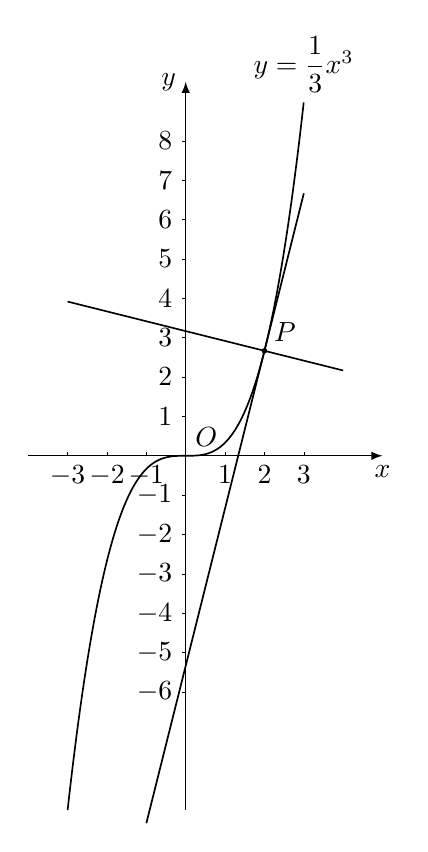
\begin{tikzpicture}[>=latex,scale=0.5]
  \draw[->](-4,0)--(5,0)node[below]{$x$};
  \draw[->](0,-9)--(0,9.5)node[left]{$y$};
  \node at (0,0)[above right]{$O$};
  \foreach \x in {-6,-5,-4,-3,-2,-1,1,2,3,4,5,6,7,8}
  {
    \draw[very thin](0,\x)--(-0.1,\x)node[left]{$\x$};
  }
  \foreach \x in {-1,-2,-3,1,2,3}
  {
    \draw[very thin](\x,0.1)--(\x,0)node[below]{$\x$};
  }
  \draw[semithick,samples=200,domain=-3:3]plot (\x,{\x*\x*\x/3.0})node[above]{$y=\dfrac{1}{3}x^3$};
  \fill(2,8/3)circle(2pt)node[above right]{$P$};
  \draw[semithick](-3,47/12)--(4,26/12)(3,20/3)--(-1,-28/3);
\end{tikzpicture}
\end{document}